\documentclass[border=3pt]{standalone}
% Preâmbulo compartilhado pelos diagramas TikZ da aula 14 (SLAM com EIF)
\usepackage[T1]{fontenc}
\usepackage[utf8]{inputenc}
\usepackage{lmodern}
\usepackage{amsmath}
\usepackage{xcolor}
\usepackage{tikz}
\usetikzlibrary{arrows.meta,angles,quotes,decorations.pathmorphing,decorations.pathreplacing,calc,
                positioning,shapes.geometric,shapes.misc,backgrounds,fit,
                math}

% Paleta (mesma dos SVGs originais)
\definecolor{dblue}{HTML}{2A5B8C}
\definecolor{dorange}{HTML}{B3541E}
\definecolor{dgreen}{HTML}{4A7C59}
\definecolor{dred}{HTML}{9C4B4B}
\definecolor{dcream}{HTML}{F4F1EA}
\definecolor{dshade}{HTML}{DDD7C9}

% Função gaussiana (não normalizada por padrão de escala visual)
\pgfmathdeclarefunction{gauss}{3}{%
  \pgfmathparse{1/(#3*sqrt(2*pi))*exp(-((#1-#2)^2)/(2*#3^2))}%
}

% Estilos comuns (prefixo d... para não colidir com chaves internas do pgf)
\tikzset{
  >={Stealth[length=2mm]},
  dguide/.style={gray!55, dashed, line width=0.4pt},
  daxis/.style={gray!60, line width=0.7pt, ->},
  dbody/.style={fill=black!3, draw=black!80, line width=1pt},
  dacc/.style={draw=dblue, line width=1pt},
  dlbl/.style={black!55, font=\small},
  dsub/.style={black!45, font=\footnotesize},
  dstate/.style={circle, draw=black!80, fill=dcream, line width=1pt,
                 minimum size=17mm, font=\large, inner sep=1pt},
  dobs/.style={circle, draw=black!80, fill=dshade, line width=1pt,
               minimum size=14mm, font=\large, inner sep=1pt},
  dbox/.style={rounded corners=2pt, draw=black!80, fill=dcream, line width=1pt,
               align=center, inner sep=6pt},
  dop/.style={circle, draw=black!80, fill=white, line width=1pt,
              minimum size=6mm, inner sep=0pt, font=\small},
  dtrans/.style={->, dblue, line width=1pt},
  dmeas/.style={->, dorange, line width=1pt},
  dcurve/.style={line width=1pt, dblue},
  dcurveb/.style={line width=1.4pt, dorange},
}

\begin{document}
\hyphenpenalty=10000 \exhyphenpenalty=10000 \tolerance=9999 \emergencystretch=3em
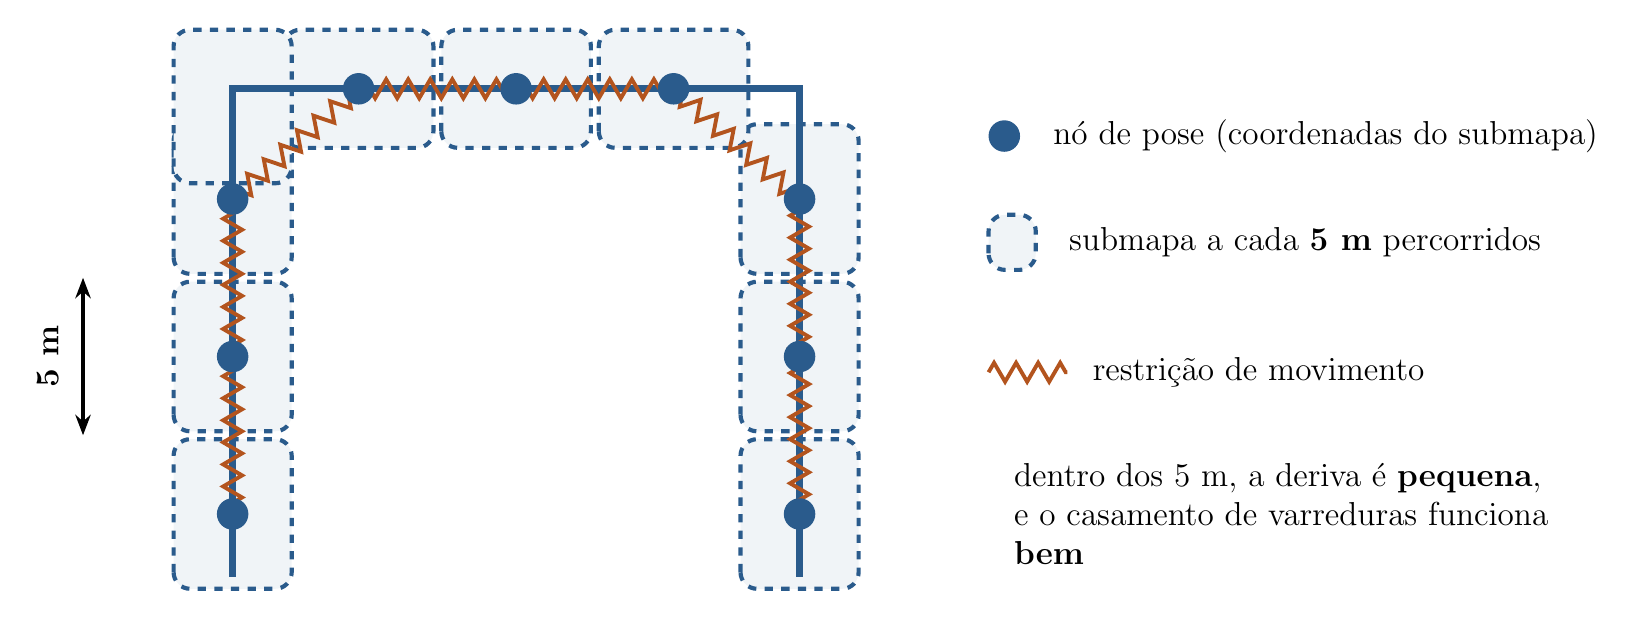
\begin{tikzpicture}[x=1cm,y=1cm]
\tikzset{sub/.style={draw=dblue, dashed, line width=1.5pt, fill=dblue!7, rounded corners=6pt},
        sp/.style={decorate, decoration={zigzag, segment length=2.8mm, amplitude=1.2mm}, line width=1.4pt, draw=dorange}}
\foreach \px/\py in {1.2/1.8,1.2/3.8,1.2/5.8,8.4/5.8,8.4/3.8,8.4/1.8} {\draw[sub] ({\px-0.75},{\py-0.95}) rectangle ({\px+0.75},{\py+0.95});}
\foreach \px/\py in {2.8/7.2,4.8/7.2,6.8/7.2} {\draw[sub] ({\px-0.95},{\py-0.75}) rectangle ({\px+0.95},{\py+0.75});}
\draw[sub] (0.45,6.0) rectangle (1.95,7.95);
\draw[dblue, line width=2.6pt] (1.2,1.0) -- (1.2,7.2) -- (8.4,7.2) -- (8.4,1.0);
\coordinate (n1) at (1.2,1.8); \coordinate (n2) at (1.2,3.8); \coordinate (n3) at (1.2,5.8); \coordinate (n4) at (2.8,7.2); \coordinate (n5) at (4.8,7.2); \coordinate (n6) at (6.8,7.2); \coordinate (n7) at (8.4,5.8); \coordinate (n8) at (8.4,3.8); \coordinate (n9) at (8.4,1.8);
\foreach \a/\b in {n1/n2,n2/n3,n3/n4,n4/n5,n5/n6,n6/n7,n7/n8,n8/n9} {\draw[sp] (\a) -- (\b);}
\foreach \k in {n1,n2,n3,n4,n5,n6,n7,n8,n9} {\fill[dblue] (\k) circle (0.2);}
\draw[line width=1.4pt, {Stealth[length=2.6mm]}-{Stealth[length=2.6mm]}] (-0.7,2.8) -- (-0.7,4.8); \node[font=\large\bfseries, rotate=90] at (-1.15,3.8) {5 m};
\fill[dblue] (11.0,6.6) circle (0.2); \node[font=\large, anchor=west] at (11.5,6.6) {nó de pose (coordenadas do submapa)};
\draw[sub] (10.8,4.9) rectangle (11.4,5.6); \node[font=\large, anchor=west] at (11.7,5.25) {submapa a cada \textbf{5 m} percorridos};
\draw[sp] (10.8,3.6) -- (11.8,3.6); \node[font=\large, anchor=west] at (12.0,3.6) {restrição de movimento};
\node[font=\large, anchor=west, text width=7.0cm] at (11.0,1.8) {dentro dos 5 m, a deriva é \textbf{pequena}, e o casamento de varreduras funciona \textbf{bem}};
\end{tikzpicture}
\end{document}
